% Asal-usul (tidak pernah dicetak): lihat sources/outline_sources.md (Tahun 1: rebound elastik dan siklus seismik; momen seismik dan magnitudo; mekanisme fokal; pengukuran geodetik deformasi aktif; hukum Gutenberg--Richter). Nilai soal latihan dan soal dari kalkulator skrap Buku 3 calc/ch18.py; data gambar dari figdata/bachelor-1/gutenberg_richter.py, beachballs.py dan interseismic.py. Fokus, episentrum, magnitudo, intensitas dan seismometer dimiliki oleh Buku 1 kelas 7 (magnitudo dibangun ulang di sini sebagai magnitudo momen); gelombang P dan S oleh Buku 2 kelas 11; jenis sesar dan rake oleh bab 17; tegangan, Coulomb dan lapisan seismogenik oleh bab 16; modulus geser oleh fisika. Interferometri radar dan proyeksi stereografik termasuk dalam volume kemudian (diceritakan, tidak didefinisikan).
\chapter{Sumber gempa bumi}\label{ch:b1:earthquake-source}

% ledger: pp1515:1906, reid:1910
Pada pagi 18 April 1906, tanah di utara dan selatan San Francisco pecah sepanjang garis lebih dari empat ratus kilometer. Jalan, pagar dan deretan pohon yang melintasi garis itu terpotong, dan kedua belahan masing-masing ditemukan terpisah beberapa meter, belahan barat selalu bergeser ke utara. Juru ukur telah mengukur posisi patok-patok di wilayah itu selama setengah abad sebelumnya, dan ketika patok-patok itu diukur lagi perbandingannya menunjukkan sesuatu yang lebih aneh daripada patahannya sendiri: tanah telah melengkung, perlahan dan mulus, selama puluhan tahun sebelum gempa, dan gempa itu membiarkannya kembali memental. Bab ini mengikuti sebuah gempa bumi dari pembebanan lambat sebuah sesar hingga beberapa menit ketika ia tergelincir, dan membaca kembali besarnya pergeseran dari gelombang dan dari tanah: seberapa besar ia, ke arah mana ia bergerak, seberapa cepat yang berikutnya sedang dipersiapkan, dan seberapa sering gempa dari setiap ukuran datang.

\begin{recall}
Fokus gempa bumi adalah titik tempat rekahan dimulai, episentrumnya titik di permukaan di atasnya; magnitudo mengukur ukuran gempa bumi, intensitas guncangan di suatu tempat; seismometer merekam gerakan tanah sebagai seismogram (Buku 1, kelas 7). Gelombang P, gelombang kompresi, datang lebih dahulu dan gelombang S, gelombang geser, sesudahnya (Buku 2, kelas 11). Sebuah sesar memiliki \omterm{def:b1:faults-folds-fabrics:fault-elements}{dinding gantung} dan \omterm{def:b1:faults-folds-fabrics:fault-elements}{dinding bawah}; \omterm{def:b1:faults-folds-fabrics:fault-elements}{vektor geser} adalah pergeseran \omterm{def:b1:faults-folds-fabrics:fault-elements}{dinding gantung} relatif terhadap \omterm{def:b1:faults-folds-fabrics:fault-elements}{dinding bawah}, \omterm{def:b1:faults-folds-fabrics:fault-elements}{rake-nya} $r$ diukur pada bidang sesar dari \omterm{def:b1:geological-maps:attitude}{jurus}, dan \omterm{def:b1:faults-folds-fabrics:fault-elements}{rake} menamai sesar: sekitar \ang{90} \omterm{def:b1:faults-folds-fabrics:fault-types}{sesar naik}, sekitar \ang{-90} \omterm{def:b1:faults-folds-fabrics:fault-types}{sesar normal}, sekitar 0 sesar \omterm{def:b1:faults-folds-fabrics:fault-types}{sinistral}, sekitar \ang{180} sesar \omterm{def:b1:faults-folds-fabrics:fault-types}{dekstral} (\cref{ch:b1:faults-folds-fabrics}). Padatan elastik kembali ke bentuknya ketika tegangan dihilangkan; modulus geser $\mu$ menghubungkan tegangan geser dengan \omterm{def:b1:stress-strain-rheology:strain}{regangan geser} yang dihasilkannya (fisika); sesar tergelincir ketika tegangan geser mencapai kekuatan geseknya, dan gempa bumi dimulai di bagian atas rapuh \omterm{def:b1:layered-earth:layers}{kerak}, \omterm{def:b1:stress-strain-rheology:strength-envelope}{lapisan seismogenik} (\cref{ch:b1:stress-strain-rheology}). Stasiun penentuan posisi satelit permanen, yang posisi hariannya selama bertahun-tahun memberi kecepatan tanah tempat mereka berdiri, mengukur gerak lempeng (\cref{ch:b1:plate-kinematics}).
\end{recall}

\section{Rebound elastik dan siklus seismik}\label{sec:b1:earthquake-source:cycle}

Dua lempeng yang saling tergelincir pada laju mantap tidak, secara umum, tergelincir secara mantap sepanjang sesar di antara keduanya. Gesekan mengunci sesar sementara lempeng terus bergerak jauh darinya, sehingga batuan di kedua sisinya melengkung seperti pegas. Ketika tegangan geser pada sesar mencapai kekuatannya, sesar tergelincir dalam beberapa detik atau menit, dan batuan yang melengkung itu memental kembali.

\begin{definition}[Rebound elastik, siklus seismik, interval perulangan]\label{def:b1:earthquake-source:seismic-cycle}
\emph{Rebound elastik}\index{rebound elastik} adalah kembalinya mendadak ke arah bentuk tanpa regangan oleh batuan di kedua sisi sebuah sesar, ketika sesar, yang terkunci selama mereka tertegangi, tergelincir dalam gempa bumi; energi elastik yang tersimpan di dalamnya dilepaskan, sebagian sebagai gelombang seismik. \emph{Siklus seismik}\index{siklus seismik} sebuah segmen sesar adalah urutan berulang dari tahap antaseismik yang panjang, ketika segmen terkunci dan regangan terkumpul di sekitarnya, tahap koseismik, gempa bumi itu sendiri, ketika ia tergelincir, dan tahap pascaseismik, berbulan-bulan hingga puluhan tahun, ketika sekitarnya menyesuaikan diri dengan keadaan baru. \emph{Interval perulangan}\index{interval perulangan} sebuah segmen adalah waktu antara dua gempa bumi besar yang berurutan di atasnya.
\end{definition}
% ledger: usgs:gloss-rebound, reid:1910, usgs:pp1515-thatcher

\begin{omfigure}
\begin{tikzpicture}[>={Stealth[length=5pt]}, font=\small]
% map view of a fence across a locked dextral strike-slip fault (north up): (a) built straight;
% (b) after decades of loading, bent with the interseismic profile v(x) = -(s/pi) arctan(x/D)
% (dextral: the east side moves south); (c) after the earthquake, straight again on each side and
% offset by s at the fault. Panel 3.4 cm wide (x from -1.7 to 1.7 cm), D = 0.35 cm, s = 0.9 cm.
\def\s{0.9}\def\Dl{0.35}
\foreach \k/\t in {0/{(a) pagar dibangun}, 1/{(b) puluhan tahun pembebanan}, 2/{(c) setelah gempa bumi}} {
  \begin{scope}[xshift=\k*4.6cm]
    \fill[omLithSand!25] (-1.7,-1.6) rectangle (1.7,1.6);
    \draw[black!50, line width=0.4pt] (-1.7,-1.6) rectangle (1.7,1.6);
    \draw[fault, line width=1.1pt] (0,-1.6) -- (0,1.6);
    \node[anchor=north, align=center, font=\scriptsize] at (0,-1.7) {\t};
    % far-field motion of the two blocks, relative to the fault
    \draw[->, omThm, line width=0.8pt] (-1.35,-1.25) -- (-1.35,-0.45);
    \draw[->, omThm, line width=0.8pt] (1.35,1.25) -- (1.35,0.45);
    \ifnum\k=0
      \draw[line width=1.2pt, omDef] (-1.7,0) -- (1.7,0);
    \fi
    \ifnum\k=1
      \draw[line width=1.2pt, omDef] plot[domain=-1.7:1.7, samples=81, variable=\x] (\x, {-\s/pi*atan(\x/\Dl)*pi/180});
      \draw[black!45, dashed, line width=0.4pt] (-1.7,0) -- (1.7,0);
    \fi
    \ifnum\k=2
      \draw[line width=1.2pt, omDef] (-1.7,{\s/2}) -- (0,{\s/2});
      \draw[line width=1.2pt, omDef] (0,{-\s/2}) -- (1.7,{-\s/2});
      \draw[black!45, dashed, line width=0.4pt] (-1.7,0) -- (1.7,0);
      \draw[<->, line width=0.5pt] (0.18,{\s/2}) -- (0.18,{-\s/2});
      \node[anchor=west, font=\scriptsize] at (0.2,0.12) {pergeseran};
    \fi
  \end{scope}
}
\node[anchor=south, font=\scriptsize] at (0,1.62) {sesar};
\draw[->, line width=0.5pt] (-1.5,0.75) -- (-1.5,1.15) node[above, font=\scriptsize, inner sep=1pt] {U};
\end{tikzpicture}
\par\smallskip{\small \omterm{def:b1:earthquake-source:seismic-cycle}{Rebound elastik} dilihat dari atas, pada sebuah pagar (biru) yang dibangun lurus melintasi \omterm{def:b1:faults-folds-fabrics:fault-types}{sesar geser-mendatar} \omterm{def:b1:faults-folds-fabrics:fault-types}{dekstral} yang terkunci. Panah merah: gerak kedua blok jauh dari sesar, relatif terhadapnya. (b) Selama sesar terkunci, tanah jauh bergerak dan pagar melengkung, sepanjang kurva profil antarseismik \cref{sec:b1:earthquake-source:geodesy}. (c) Gempa bumi melepaskan lengkungan itu: setiap belahan pagar lurus kembali, dan kedua belahan bergeser di sesar sebesar pergeseran itu. Lengkungan itu dibesar-besarkan: pagar sungguhan melengkung beberapa meter sepanjang puluhan kilometer.}
\label{fig:b1:earthquake-source:rebound}
\end{omfigure}

Jika sesar terkunci di antara gempa bumi dan setiap gempa bumi membatalkan pergeseran yang telah dikumpulkan lempeng sejak yang terakhir, gerak lempeng menentukan laju siklusnya.

\begin{proposition}[Perulangan dari laju pergeseran]\label{prop:b1:earthquake-source:recurrence}
Misalkan sebuah segmen sesar dibebani pada laju pergeseran jangka panjang $\dot s$, terkunci di antara gempa bumi, dan tergelincir sebesar jumlah yang sama $D$ pada setiap gempa bumi. Maka \omterm{def:b1:earthquake-source:seismic-cycle}{interval perulangan} gempa-gempanya adalah
\[
  T = \frac{D}{\dot s} .
\]
Jika hanya fraksi $c$ dari laju pergeseran yang terkunci, sisanya tergelincir mantap tanpa gempa bumi, $T = D/(c\,\dot s)$.
\end{proposition}

\begin{proof}
Selama waktu panjang $t$, kedua sisi sesar bergerak sebesar $\dot s\,t$ relatif satu sama lain. Jauh dari sesar tanah bergerak mantap, sehingga pada sesar itu sendiri pergeseran yang sama harus dipenuhi, di sini oleh gempa bumi saja: jika $N$ gempa bumi terjadi dalam waktu $t$, maka $N D = \dot s\,t$ hingga pergeseran satu gempa bumi, dan $t/N \to D/\dot s$. Dengan fraksi $1-c$ dari pergeseran dibuat oleh peluncuran mantap, gempa bumi memenuhi $c\,\dot s\,t$ dan $t/N \to D/(c\,\dot s)$.
\end{proof}

Dengan nilai yang khas bagi sesar San Andreas, pergeseran \qty{4}{m} pada setiap gempa bumi besar dan laju pergeseran \qty{20}{mm.yr^{-1}}, \omterm{def:b1:earthquake-source:seismic-cycle}{interval perulangannya} adalah \qty{200}{yr}. Di Wallace Creek, di California tengah, sebuah alur sungai yang terpotong melintasi sesar telah tergeser sebesar \qty{128}{m} dalam \num{3587} tahun sejak ia tergerus, rata-rata \qty{36}{mm.yr^{-1}}, dekat dengan laju sekitar \qty{34}{mm.yr^{-1}} yang diukur pada pergeseran lain di sana; gempa bumi besar terakhir di bentangan itu, pada 1857, tergelincir hampir \qty{10}{m}, yang pada laju ini memerlukan sekitar tiga abad untuk terkumpul.
% ledger: usgs:pp1515-thatcher, usgs:pp1515-wallace, commons:wallace-creek

\begin{omfigure}
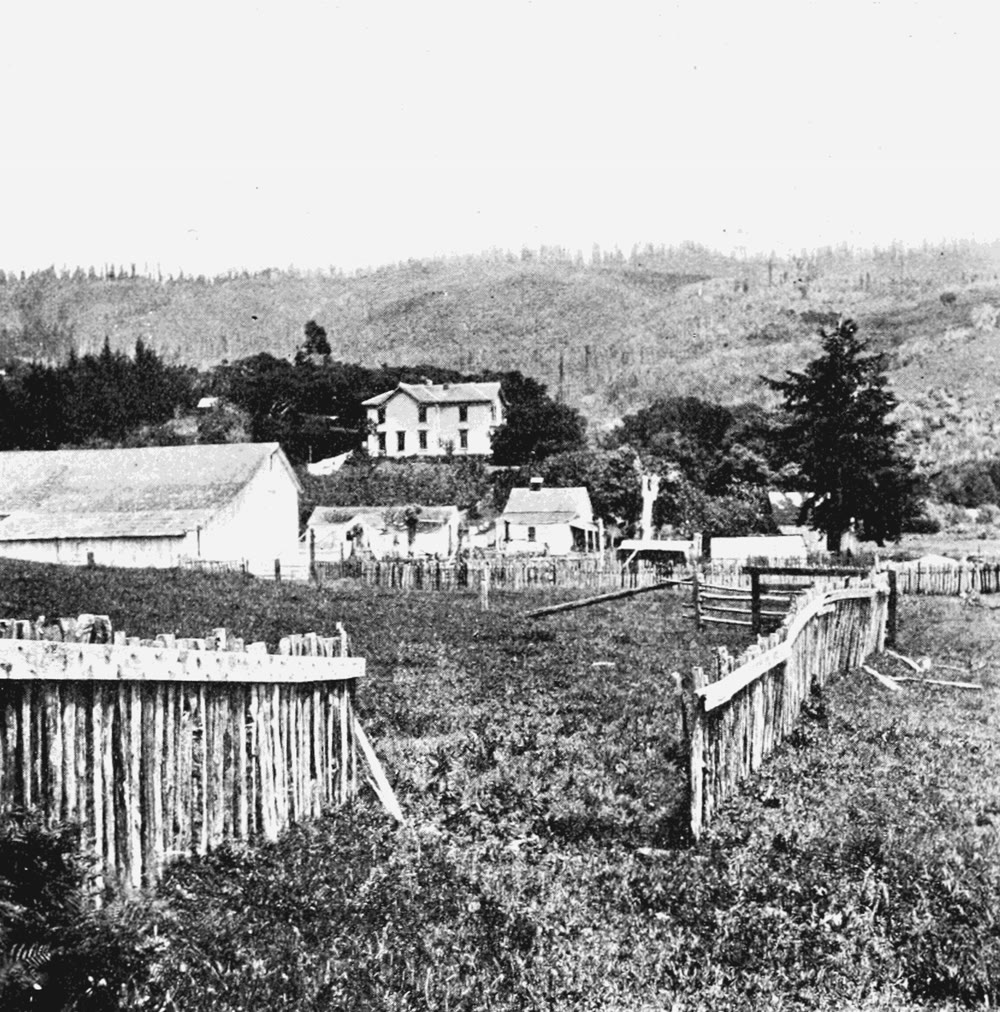
\includegraphics[height=5.6cm]{images/book3/b1-fence-1906.jpg}\hfill
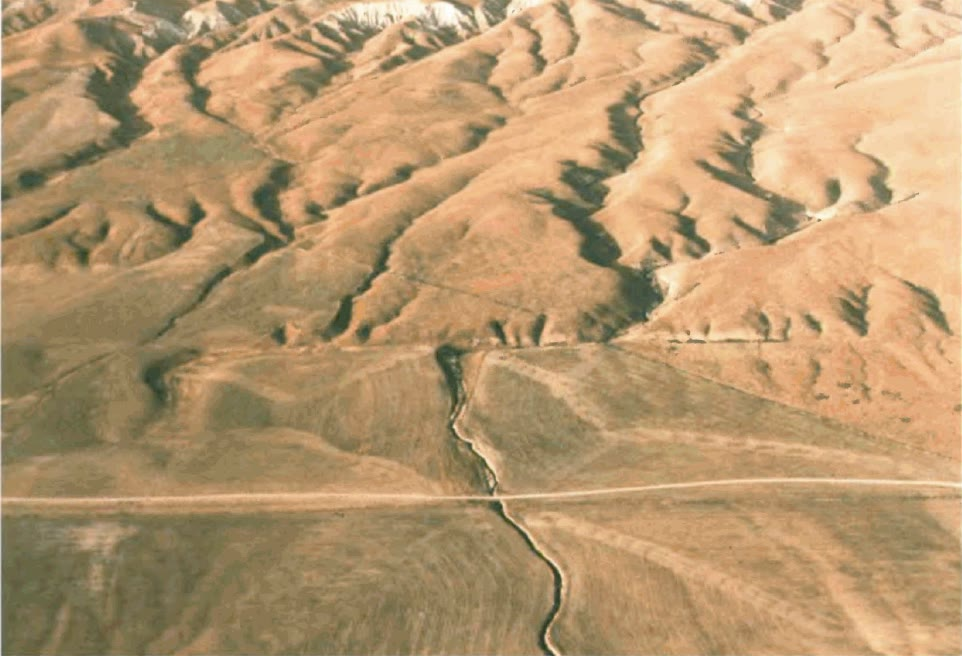
\includegraphics[height=5.6cm]{images/book3/b1-wallace-creek.jpg}
\par\smallskip{\small Kiri: pagar di lahan pertanian Marin County, di utara San Francisco, yang dilintasi rekahan 1906, diterbitkan tahun yang sama sebagai ``tanah yang terpisah oleh sesar gempa bumi''. Foto dari \emph{Popular Science Monthly}, jilid~69 (1906), domain publik. Kanan: Wallace Creek, Carrizo Plain, dilihat dari udara: sungai turun dari bukit-bukit (atas), dan tempat ia memotong sesar San Andreas, di kaki bukit, alurnya bergeser ke samping sebesar \qty{130}{m}, pergeseran yang terkumpul selama ribuan tahun gempa bumi. Foto: R.~E.~Wallace, U.S. Geological Survey, domain publik. Keduanya dari Wikimedia
Commons.}
\label{fig:b1:earthquake-source:offsets}
\end{omfigure}
% ledger: commons:psm-fence, commons:wallace-creek

Proposisi memberi rata-rata, bukan jadwal. Di dekat Parkfield, pada sesar yang sama, sebuah gempa bumi berkekuatan sekitar 6 pada 1857 diikuti oleh lima lainnya, yang sangat mirip, pada bentangan yang sama sepanjang sekitar \qty{30}{km}, dengan interval hampir 22 tahun hingga 1966; yang berikutnya diharapkan sebelum 1993, dan datang pada 2004, dengan \omterm{def:b1:earthquake-source:mw}{magnitudo momen} 6.0 dan tanpa tanda peringatan yang jelas. Kekuatan sebuah sesar, pergeseran setiap gempa bumi dan pembebanan oleh tetangganya semuanya bervariasi dari satu siklus ke siklus berikutnya, dan \omterm{def:b1:earthquake-source:seismic-cycle}{siklus seismik} lebih baik digambarkan oleh \omterm{def:b1:earthquake-source:seismic-cycle}{interval perulangan} rata-rata dan sebaran di sekitarnya daripada oleh suatu periode.
% ledger: pp1515:parkfield, bl85:parkfield, usgs:hist-mw, bakun:2005

Beberapa segmen sesar tidak terkunci sama sekali. Di antara Parkfield dan San Juan Bautista, bagian tengah sesar San Andreas merayap: peluncuran mantap pada sesar menampung hampir seluruh gerak lempeng, dan sedikit jika ada regangan terkumpul di kedua sisinya, sehingga bagian ini tidak memiliki gempa bumi besar; gempa bumi besar 1857 dimulai di ujung selatannya dan yang 1906 berhenti di ujung utaranya. Sebuah sesar yang merayap pada sebagian areanya hanya terkunci sebagian, yaitu koefisien $c$ dalam proposisi.
% ledger: pp1515:creep, pp1515:1906

\begin{inthefield}[Membaca gempa bumi masa lalu dalam parit]
Instrumen telah merekam gempa bumi selama tidak lebih dari satu abad, jauh lebih sedikit daripada satu siklus sebagian besar sesar. Paleoseismolog memperpanjang catatan dengan membaca tanah. Sebuah parit setebal beberapa meter digali melintasi sesar aktif tempat lapisan sedimen diendapkan secara menerus, di rawa, danau atau kipas aluvium kecil. Di dinding-dindingnya, setiap gempa bumi tampak sebagai lapisan yang terpotong dan tergeser oleh sesar dan tertutup, tanpa retak, oleh lapisan yang lebih muda; sebagai tebing yang terkubur oleh endapan kemudian; sebagai pasir yang mencair dan naik melalui retakan untuk menyebar di permukaan pada saat itu. Sisa gambut atau tumbuhan dalam lapisan tepat di bawah dan di atas setiap patahan diberi tanggal dengan radiokarbon, dan dengan demikian membatasi tanggal setiap gempa bumi: satu rawa pada sesar San Andreas menyimpan catatan dua belas. Di sepanjang pantai, lembaran pasir yang diendapkan oleh tsunami dan rawa yang tenggelam mendadak sekitar satu meter, terkubur di bawah lumpur pasang, mencatat gempa bumi subduksi besar. Pada sesar San Andreas, sebagian besar pergeseran pada masa sejarah datang bersama gempa bumi bermagnitudo 6 atau lebih.
\end{inthefield}
% ledger: pp1515:pallett, atwater:1987

\begin{history}[Harry Fielding Reid dan rebound elastik]
Harry Fielding Reid, fisikawan Amerika, adalah anggota komisi negara bagian yang mempelajari gempa bumi 1906. Dengan membandingkan posisi titik-titik yang disurvei pada 1851--1865, pada 1874--1892 dan setelah gempa bumi, ia mendapati bahwa titik-titik jauh di kedua sisi sesar San Andreas telah bergeser sekitar \qty{3.2}{m} relatif satu sama lain sejak survei pertama, sedikit lebih dari separuh pergeseran sekitar \qty{6}{m} pada sesar itu: setengah abad sebelum gempa bumi, regangan yang mematahkan sesar itu sudah separuh terbangun. Hanya gaya elastik yang dapat menggerakkan tanah sedemikian mendadak, dan ia menamai kembalinya mendadak itu \omterm{def:b1:earthquake-source:seismic-cycle}{rebound elastik}. Ia menerbitkannya dalam jilid kedua
laporan komisi, pada 1910; ia masih menjadi model utama siklus gempa bumi. Penentuan posisi satelit sejak itu mengukur lengkungan yang hanya bisa ia simpulkan.
\end{history}
% ledger: reid:1910, pp1515:1906

\section{Momen seismik dan magnitudo}\label{sec:b1:earthquake-source:moment}

Ukuran sebuah gempa bumi adalah jumlah pergeseran yang dibuatnya, atas luas sesar yang tergelincir, dikalikan dengan seberapa kaku batuannya.

\begin{definition}[Momen seismik]\label{def:b1:earthquake-source:moment}
Misalkan sebuah gempa bumi bergeser sebesar rata-rata $D$ atas rekahan seluas $A$, di dalam batuan dengan modulus geser $\mu$ (huruf ini juga menamai koefisien gesekan, dalam \cref{ch:b1:stress-strain-rheology}; konteks yang menunjukkan yang mana). \emph{Momen seismik}\index{momen seismik} adalah
\[
  M_0 = \mu A D ,
\]
dalam newton meter.
\end{definition}
% ledger: usgs:gloss-moment

Satuannya adalah satuan torsi. Pergeseran pada sesar mengirimkan gelombang yang sama dengan dua pasang gaya berlawanan, dua kopel, yang diterapkan di fokus, dan \omterm{def:b1:earthquake-source:moment}{momen seismik} adalah momen setiap kopel itu (ekuivalensi ini, kopel ganda, dibuktikan dalam volume Tahun ke-3). Momen memiliki dimensi energi, tetapi ia bukan energi: energi yang dipancarkan sebagai gelombang hanyalah sebagian kecil darinya. Untuk batuan \omterm{def:b1:layered-earth:layers}{kerak}, $\mu$ diambil sebesar \qty{30}{GPa}.
% ledger: kanamori:1977, sk:mu-locking

Momen dihitung hari ini dari gelombang periode panjang yang direkam di seluruh dunia. Untuk gempa Tohoku 11 Maret 2011, solusi pilihan Survei Geologi Amerika Serikat memberi $M_0 = \qty{5.59e22}{N.m}$. Sesar tergelincir atas luas sekitar \qty{400}{km} panjangnya dan \qty{150}{km} lebarnya; definisinya kemudian memberi pergeseran rata-rata
\[
  D = \frac{M_0}{\mu A}
    = \frac{\num{5.59e22}}{\num{3e10}\times\num{4e5}\times\num{1.5e5}}
    \approx \qty{31}{m} ,
\]
dan model rekahan menemukan hingga \qtyrange{50}{60}{m} pada bagian yang paling bergeser.
% ledger: usgs:tohoku-mt, usgs:tohoku-summary

Magnitudo Buku 1 dihitung dari amplitudo gelombang pada seismogram. Magnitudo seperti itu mengukur gelombang dari satu periode; begitu sebuah rekahan jauh lebih panjang daripada panjang gelombangnya, beberapa hingga sekitar lima puluh kilometer, amplitudonya berhenti tumbuh bersama ukurannya, dan magnitudo menjadi jenuh. Magnitudo gelombang badan jenuh di sekitar 6.5, magnitudo gelombang permukaan di sekitar 8.3. Pada 2011, peringatan tsunami pertama untuk Tohoku didasarkan pada magnitudo jenis ini, yang kurang untuk gempa bumi bermagnitudo 8 atau lebih, dan ia meremehkan gelombangnya. Momen tidak jenuh, dan magnitudo kini didefinisikan darinya.
% ledger: kanamori:1977, usgs:magtypes, jma:warning

\begin{definition}[Magnitudo momen]\label{def:b1:earthquake-source:mw}
\emph{Magnitudo momen}\index{magnitudo momen} sebuah gempa bumi dengan \omterm{def:b1:earthquake-source:moment}{momen seismik} $M_0$, dalam newton meter, adalah
\[
  M_w = \tfrac23\left(\log_{10} M_0 - 9.1\right) .
\]
\end{definition}
% ledger: usgs:magtypes

Thomas Hanks dan Hiroo Kanamori mendefinisikan skala itu pada 1979, dengan konstanta 9.05 alih-alih 9.1, selisih 0.03 dalam $M_w$; konstanta-konstanta itu dipilih agar cocok dengan magnitudo lama di tempat yang tidak jenuh. Magnitudo Buku 1 untuk gempa besar adalah angka ini: untuk Tohoku,
$M_w = \tfrac23(\log_{10}\num{5.59e22} - 9.1) = \tfrac23(22.75 - 9.1) = 9.1$;
gempa Chili besar 1960 dan gempa Alaska 1964 memiliki \omterm{def:b1:earthquake-source:mw}{magnitudo momen} 9.5 dan 9.2, ukuran yang tidak dapat ditunjukkan magnitudo lama.
% ledger: hk:1979, kanamori:1977, usgs:hist-mw, usgs:tohoku-mt

\begin{proposition}[Satu satuan magnitudo]\label{prop:b1:earthquake-source:moment-steps}
\omterm{def:b1:earthquake-source:moment}{Momen seismik} adalah $M_0 = 10^{1.5 M_w + 9.1}$ newton meter. Satu satuan \omterm{def:b1:earthquake-source:mw}{magnitudo momen} mengalikannya dengan $10^{1.5} \approx 31.6$, dua satuan dengan $1000$. Jika energi yang dipancarkan adalah fraksi tetap dari momen, ia tumbuh dalam perbandingan yang sama.
\end{proposition}

\begin{proof}
Menyelesaikan definisi untuk $M_0$ memberi $\log_{10} M_0 = 1.5 M_w + 9.1$, dan untuk dua gempa bumi
\[
  \log_{10}\frac{M_0'}{M_0} = 1.5\,(M_w' - M_w) ,
\]
yang berarti $1.5$ untuk satu satuan dan $3$ untuk dua. Jika energi yang dipancarkan adalah $E_s = k M_0$ dengan $k$ yang sama untuk keduanya, $E_s'/E_s = M_0'/M_0$.
\end{proof}

Pendekatan Kanamori, $E_s \approx M_0/(2\times10^4)$ (diterima tanpa bukti), adalah anggapan kalimat terakhir; faktor sekitar 32 dalam energi per satuan magnitudo, yang ditemui di Buku 1, adalah proposisi ini. Karena $M_0 = \mu A D$ dan pergeseran sebuah gempa bumi tumbuh bersama ukuran rekahannya, magnitudo besar memerlukan sesar besar. Rekahan 1906, sepanjang sekitar \qty{430}{km}, memecah \omterm{def:b1:stress-strain-rheology:strength-envelope}{lapisan seismogenik} hingga sekitar \qty{15}{km} dengan pergeseran rata-rata beberapa meter: dengan $D = \qty{4}{m}$, $M_0 = \num{3e10}\times\num{4.3e5}\times\num{1.5e4}
\times 4 = \qty{7.7e20}{N.m}$ dan $M_w = 7.9$, magnitudo katalog. Magnitudo 9 memerlukan rekahan sepanjang ratusan kilometer dan lebih dari seratus lebar, yang hanya ditawarkan oleh bidang-bidang landai dari zona subduksi.
% ledger: kanamori:1977, pp1515:1906, usgs:hist-mw, usgs:pp1515-thatcher

\section{Mekanisme fokal}\label{sec:b1:earthquake-source:focal}

Gelombang P adalah yang pertama mencapai seismometer. Gerakan pertamanya, ayunan pertama rekaman vertikal, naik di tempat gelombang datang sebagai dorongan, tanah dimampatkan dan dilemparkan menjauh dari sumber, dan turun di tempat ia datang sebagai tarikan. Di sekitar sebuah gempa bumi, dorongan dan tarikan tersusun dalam pola yang memberi orientasi sesar dan arah pergeseran.

\begin{proposition}[Tanda gerak pertama]\label{prop:b1:earthquake-source:first-motion}
Anggap sebuah sesar dengan normal ke atas $\mathbf n$ tergelincir sebesar vektor satuan $\mathbf d$ (pergeseran \omterm{def:b1:faults-folds-fabrics:fault-elements}{dinding gantung} relatif terhadap \omterm{def:b1:faults-folds-fabrics:fault-elements}{dinding bawah}). Gelombang P yang meninggalkan fokus dalam arah satuan $\mathbf x$ datang sebagai dorongan jika $(\mathbf n\cdot\mathbf x)(\mathbf d\cdot\mathbf x) > 0$ dan sebagai tarikan jika $(\mathbf n\cdot\mathbf x)(\mathbf d\cdot\mathbf x) < 0$. Dorongan dan tarikan dengan demikian mengisi empat kuadran, dipisahkan oleh bidang sesar ($\mathbf n\cdot\mathbf x = 0$) dan oleh bidang tegak lurus terhadap pergeseran ($\mathbf d\cdot\mathbf x = 0$).
\end{proposition}

\begin{proof}
Arah dengan $\mathbf n\cdot\mathbf x > 0$ menunjuk ke dalam \omterm{def:b1:faults-folds-fabrics:fault-elements}{dinding gantung}, yang bergerak sebesar $\mathbf d$ relatif terhadap \omterm{def:b1:faults-folds-fabrics:fault-elements}{dinding bawah}: batuan di depannya, tempat $\mathbf d\cdot\mathbf x > 0$, dimampatkan, dan batuan di belakangnya, tempat $\mathbf d\cdot\mathbf x < 0$, ditarik. Arah dengan $\mathbf n\cdot\mathbf x < 0$ menunjuk ke dalam \omterm{def:b1:faults-folds-fabrics:fault-elements}{dinding bawah}, yang bergerak sebesar $-\mathbf d$ relatif terhadap \omterm{def:b1:faults-folds-fabrics:fault-elements}{dinding gantung}, sehingga tandanya terbalik. Pada setiap kasus \omterm{def:b1:earthquake-source:focal-mechanism}{gerak pertama} memiliki tanda $(\mathbf n\cdot\mathbf x)(\mathbf
d\cdot\mathbf x)$.
\end{proof}

Argumen itu hanya memberi tanda. Amplitudo \omterm{def:b1:earthquake-source:focal-mechanism}{gerak pertama}, yang sebanding dengan $2(\mathbf n\cdot\mathbf x)(\mathbf d\cdot\mathbf x)$ dan karenanya terbesar pada \ang{45} dari kedua bidang dan nol di atasnya, diterima di sini (volume Tahun ke-3).

\begin{omfigure}
\begin{tikzpicture}[>={Stealth[length=5pt]}, font=\small, scale=0.95]
% map view around a vertical dextral fault striking north, the focus at the origin, rays leaving
% horizontally: pushes where (n.x)(d.x) > 0, i.e. in the NW and SE quadrants (beachballs.py,
% first_motion(0, 90, 180, x)). Stations at 20 azimuths on a circle of radius 2.3.
\fill[omThm!22] (0,0) -- (0,2.8) arc[start angle=90, end angle=180, radius=2.8] -- cycle;
\fill[omThm!22] (0,0) -- (0,-2.8) arc[start angle=270, end angle=360, radius=2.8] -- cycle;
\draw[black!40, line width=0.4pt] (0,0) circle[radius=2.8];
\draw[fault, line width=1.3pt] (0,-3.1) -- (0,3.1) node[above, font=\scriptsize] {sesar (bidang nodal)};
\draw[black, dashed, line width=0.7pt] (-3.1,0) -- (3.1,0) node[right, font=\scriptsize, align=left] {bidang\\ bantu};
% slip: the west block moves north, the east block south
\draw[->, line width=1pt] (-0.3,-0.8) -- (-0.3,0.8);
\draw[->, line width=1pt] (0.3,0.8) -- (0.3,-0.8);
% stations
\foreach \a in {9,27,...,351} {
  \pgfmathsetmacro{\fm}{-sin(\a)*cos(\a)}  % (n.x)(d.x) with n = east, d = south, x = (sin a, cos a)
  \pgfmathparse{\fm>0 ? 1 : 0}
  \ifnum\pgfmathresult=1
    \fill[black] ({2.3*sin(\a)},{2.3*cos(\a)}) circle[radius=0.11];
  \else
    \draw[black, fill=white, line width=0.6pt] ({2.3*sin(\a)},{2.3*cos(\a)}) circle[radius=0.11];
  \fi
}
% P and T axes
\draw[<-, omProp, line width=1.1pt] ({0.7*sin(45)},{0.7*cos(45)}) -- ({1.6*sin(45)},{1.6*cos(45)}) node[above right, font=\scriptsize, inner sep=1pt] {P};
\draw[<-, omProp, line width=1.1pt] ({0.7*sin(225)},{0.7*cos(225)}) -- ({1.6*sin(225)},{1.6*cos(225)});
\draw[->, omProp, line width=1.1pt] ({0.7*sin(315)},{0.7*cos(315)}) -- ({1.6*sin(315)},{1.6*cos(315)}) node[above left, font=\scriptsize, inner sep=1pt] {T};
\draw[->, omProp, line width=1.1pt] ({0.7*sin(135)},{0.7*cos(135)}) -- ({1.6*sin(135)},{1.6*cos(135)});
\fill (0,0) circle[radius=0.06];
% legend
\begin{scope}[xshift=4.6cm, yshift=2.4cm]
  \fill[black] (0,0) circle[radius=0.11]; \node[anchor=west, font=\scriptsize] at (0.2,0) {dorongan: gerak pertama ke atas};
  \draw[black, fill=white, line width=0.6pt] (0,-0.5) circle[radius=0.11]; \node[anchor=west, font=\scriptsize] at (0.2,-0.5) {tarikan: gerak pertama ke bawah};
  \fill[omThm!22] (-0.12,-1.12) rectangle (0.12,-0.88); \node[anchor=west, font=\scriptsize] at (0.2,-1.0) {kuadran kompresi};
  \draw[->] (-0.1,-1.6) -- (-0.1,-1.25); \node[anchor=west, font=\scriptsize] at (0.2,-1.42) {U};
\end{scope}
\end{tikzpicture}
\par\smallskip{\small \omterm{def:b1:earthquake-source:focal-mechanism}{Gerak pertama} di sekitar sebuah \omterm{def:b1:faults-folds-fabrics:fault-types}{sesar geser-mendatar} \omterm{def:b1:faults-folds-fabrics:fault-types}{dekstral} vertikal yang berjurus utara, dilihat dari atas, untuk gelombang yang meninggalkan fokus secara horizontal menuju stasiun-stasiun di sekelilingnya. Panah hitam: pergeseran kedua blok. Dorongan mengisi kuadran barat laut dan tenggara, tarikan dua lainnya; sesar dan \omterm{def:b1:earthquake-source:focal-mechanism}{bidang bantu} memisahkannya. \omterm{def:b1:earthquake-source:focal-mechanism}{Sumbu P} (panah yang menunjuk masuk) membagi dua kuadran tarikan, \omterm{def:b1:earthquake-source:focal-mechanism}{sumbu T} (panah yang menunjuk keluar) kuadran dorongan. Pergeseran \omterm{def:b1:faults-folds-fabrics:fault-types}{sinistral} pada bidang putus-putus, blok di selatannya bergerak ke timur, akan memberi pola yang persis sama (\cref{prop:b1:earthquake-source:auxiliary}).}
\label{fig:b1:earthquake-source:quadrants}
\end{omfigure}

Hasil kali $(\mathbf n\cdot\mathbf x)(\mathbf d\cdot\mathbf x)$ tidak berubah ketika $\mathbf n$ dan $\mathbf d$ dipertukarkan. Simetri ini adalah fakta sentral \omterm{def:b1:earthquake-source:focal-mechanism}{mekanisme fokal}.

\begin{definition}[Mekanisme fokal, bidang nodal, bidang bantu, sumbu P, sumbu T]\label{def:b1:earthquake-source:focal-mechanism}
\emph{Gerak pertama}\index{gerak pertama} sebuah gelombang P di seismometer adalah arah, naik atau turun, dari gerakan pertama tanah pada rekaman vertikal. \emph{Mekanisme fokal}\index{mekanisme fokal} sebuah gempa bumi adalah orientasi bidang sesar dan arah pergeseran di atasnya, seperti yang ditemukan dari gelombang seismiknya. Kedua bidang tegak lurus melalui fokus yang memisahkan dorongan dari tarikan adalah \emph{bidang nodalnya}\index{bidang nodal}; salah satunya adalah bidang sesar, dan yang lain, tegak lurus terhadap pergeseran, adalah \emph{bidang bantu}\index{bidang bantu}. \emph{Sumbu P}\index{sumbu P} dan \emph{sumbu T}\index{sumbu T} adalah arah pada \ang{45} dari kedua bidang nodal di tengah kuadran tarikan dan kuadran dorongan:
\[
  \mathbf P = \frac{\mathbf n - \mathbf d}{\sqrt2}, \qquad
  \mathbf T = \frac{\mathbf n + \mathbf d}{\sqrt2} .
\]
\end{definition}
% ledger: yvo:beachball, usgs:gloss-moment

\begin{proposition}[Dua bidang nodal]\label{prop:b1:earthquake-source:auxiliary}
Pergeseran $\mathbf d$ pada bidang dengan normal $\mathbf n$ dan pergeseran $\mathbf n$ pada bidang dengan normal $\mathbf d$ memberi \omterm{def:b1:earthquake-source:focal-mechanism}{gerak pertama} yang sama di setiap arah. \omterm{def:b1:earthquake-source:focal-mechanism}{Gerak pertama} karenanya menentukan kedua \omterm{def:b1:earthquake-source:focal-mechanism}{bidang nodal}, \omterm{def:b1:earthquake-source:focal-mechanism}{sumbu P} dan T serta arah pergeseran pada setiap bidang, tetapi tidak memberi tahu \omterm{def:b1:earthquake-source:focal-mechanism}{bidang nodal} mana yang merupakan sesar.
\end{proposition}

\begin{proof}
Tanda $(\mathbf n\cdot\mathbf x)(\mathbf d\cdot\mathbf x)$ tidak berubah oleh pertukaran $\mathbf n$ dan $\mathbf d$; bidang-bidang $\mathbf n\cdot\mathbf x = 0$ dan $\mathbf d\cdot\mathbf x = 0$ saling dipertukarkan,
dan $\mathbf n \pm \mathbf d$ tidak berubah. Pasangan $(\mathbf n, \mathbf d)$ dan
pasangan $(-\mathbf n, -\mathbf d)$, yang menggambarkan pergeseran yang sama dilihat dari blok lain, juga memberi hasil kali yang sama. Tidak ada yang di dalam \omterm{def:b1:earthquake-source:focal-mechanism}{gerak pertama} membedakan kedua deskripsi itu.
\end{proof}

Untuk memutuskan \omterm{def:b1:earthquake-source:focal-mechanism}{bidang nodal} mana yang tergelincir, seismolog memakai bukti lain: bidang sepanjang gempa susulan berbaris, sesar yang terlihat di permukaan, batas lempeng tempat gempa bumi itu terletak. Untuk gempa Sumatra--Andaman besar 2004, kedua \omterm{def:b1:earthquake-source:focal-mechanism}{bidang nodal} miring \ang{8} ke timur laut dan \ang{83} ke barat daya. Gempa-gempa terdahulu di wilayah itu dan model lempeng keduanya menempatkan \omterm{def:b1:active-margins:slab}{slab yang menunjam} sepanjang bidang yang miring landai ke timur laut, dan bidang dangkal diambil sebagai sesar: gempa bumi itu memecah antarmuka lempeng zona subduksi, dan gempa susulannya tersebar lebih dari \qty{1300}{km}.
% ledger: usgs:sumatra-mt, usgs:sumatra-summary

Karena \omterm{def:b1:earthquake-source:focal-mechanism}{sumbu P} terletak di tengah tarikan dan \omterm{def:b1:earthquake-source:focal-mechanism}{sumbu T} di tengah dorongan, keduanya sering dibaca sebagai arah tegangan tekan terbesar dan terkecil, $\sigma_1$ dan $\sigma_3$. Itu hanya perkiraan. Sesar baru terbentuk pada $\ang{45} - \phi/2$ dari $\sigma_1$, bukan pada \ang{45} (\cref{ch:b1:stress-strain-rheology}), dan sesar lama mungkin tergelincir pada sudut yang masih berbeda, sehingga sumbu satu gempa bumi dapat berada puluhan derajat dari \omterm{def:b1:stress-strain-rheology:principal}{tegangan utama}; tegangan suatu wilayah ditemukan dari mekanisme banyak gempa bumi bersama-sama.

\omterm{def:b1:earthquake-source:focal-mechanism}{Mekanisme fokal} hidup pada bola di sekitar fokus. Ia digambar pada belahan bawah bola itu, yang dilintasi setiap sinar menuju stasiun jauh, diproyeksikan ke sebuah cakram: sinar dengan vektor satuan $\mathbf x = (E, N, U)$, dengan $U \le 0$, diplot pada
\[
  (X, Y) = \frac{(E, N)}{\sqrt{1 - U}} ,
\]
vertikal di pusat dan horizontal pada lingkaran satuan. Proyeksi ini mempertahankan luas (diterima; proyeksi bola dipelajari dalam volume Tahun ke-3), sehingga setiap kuadran menutupi bagian sejatinya dari cakram. Kuadran dorongan diarsir; gambarnya disebut bola pantai.
% ledger: yvo:beachball

\begin{omfigure}
\begin{tikzpicture}[font=\small]
% lower-hemisphere equal-area beach balls, compressional quadrants shaded (figdata/bachelor-1/beachballs.py)
\foreach \n/\c/\t/\x in {normal/2/{(a) sesar normal\\ $090/60$, rake \ang{-90}}/0,
                         reverse/1/{(b) sesar naik\\ $090/30$, rake \ang{90}}/3.65,
                         strikeslip/2/{(c) sesar geser-mendatar\\ $090/90$, rake \ang{180}}/7.3,
                         tohoku/2/{(d) Tohoku, 2011\\ $282/8$, rake \ang{78}}/10.95} {
  \begin{axis}[at={(\x cm,0)}, anchor=center, width=2.9cm, height=2.9cm, scale only axis,
      axis equal image, xmin=-1.04, xmax=1.04, ymin=-1.04, ymax=1.04, hide axis, clip=false]
    \fill[white] (axis cs:0,0) circle[radius=1];
    \addplot[fill=omThm!55, draw=none] table[x=X, y=Y] {figdata/out/bachelor-1-beachballs-\n-c1.dat};
    \ifnum\c=2
      \addplot[fill=omThm!55, draw=none] table[x=X, y=Y] {figdata/out/bachelor-1-beachballs-\n-c2.dat};
    \fi
    \addplot[black, line width=0.6pt] table[x=X, y=Y] {figdata/out/bachelor-1-beachballs-\n-p1.dat};
    \addplot[black, line width=0.6pt] table[x=X, y=Y] {figdata/out/bachelor-1-beachballs-\n-p2.dat};
    \draw[black, line width=0.8pt] (axis cs:0,0) circle[radius=1];
    \draw[black, line width=0.5pt] (axis cs:0,1) -- (axis cs:0,1.12) node[above, font=\scriptsize, inner sep=1pt] {U};
    \addplot[only marks, mark=none, nodes near coords={\textbf{P}}, nodes near coords align=center, every node near coord/.append style={font=\scriptsize, inner sep=0pt}] table[x=X, y=Y] {figdata/out/bachelor-1-beachballs-\n-P.dat};
    \addplot[only marks, mark=none, nodes near coords={\textbf{T}}, nodes near coords align=center, every node near coord/.append style={font=\scriptsize, inner sep=0pt}] table[x=X, y=Y] {figdata/out/bachelor-1-beachballs-\n-T.dat};
    \node[anchor=north, align=center, font=\scriptsize] at (axis cs:0,-1.12) {\t};
  \end{axis}
}
\end{tikzpicture}
\par\smallskip{\small Bola pantai: belahan bawah di sekitar fokus dalam proyeksi luas-sama, utara ke atas, kuadran dorongan diarsir, P dan T menandai sumbu (sebuah huruf digeser ke dalam jika sumbunya dekat tepi). Setiap mekanisme diberikan oleh sikap satu \omterm{def:b1:earthquake-source:focal-mechanism}{bidang nodal}, \omterm{def:b1:geological-maps:attitude}{arah kemiringan} dan \omterm{def:b1:geological-maps:attitude}{kemiringannya}, serta \omterm{def:b1:faults-folds-fabrics:fault-elements}{rake} pergeseran di atasnya. (a) \omterm{def:b1:faults-folds-fabrics:fault-types}{Sesar normal} yang miring \ang{60} ke timur: kuadran tarikan mengisi pusat. (b) \omterm{def:b1:faults-folds-fabrics:fault-types}{Sesar naik} yang miring \ang{30} ke timur: kuadran dorongan mengisi pusat. (c) \omterm{def:b1:faults-folds-fabrics:fault-types}{Sesar geser-mendatar} vertikal: empat kuadran bertemu di pusat. (d) Gempa bumi Tohoku 2011 (momen tensor Survei Geologi Amerika Serikat): \omterm{def:b1:faults-folds-fabrics:fault-types}{sesar naik} pada bidang yang miring \ang{8} ke arah $282$, di bawah Jepang, dengan \omterm{def:b1:earthquake-source:focal-mechanism}{bidang bantu} curam di timur.}
\label{fig:b1:earthquake-source:beachballs}
\end{omfigure}
% ledger: usgs:tohoku-mt

Seismolog memberikan mekanisme dengan \omterm{def:b1:geological-maps:attitude}{jurus}, \omterm{def:b1:geological-maps:attitude}{kemiringan} dan \omterm{def:b1:faults-folds-fabrics:fault-elements}{rake} setiap \omterm{def:b1:earthquake-source:focal-mechanism}{bidang nodal}; \omterm{def:b1:geological-maps:attitude}{jurusnya} adalah \omterm{def:b1:geological-maps:attitude}{arah kemiringan} dikurangi \ang{90}, seperti di \cref{ch:b1:faults-folds-fabrics}. Untuk Tohoku, bidang-bidangnya adalah $192/8/78$ dan $24/81/91$ dalam \omterm{def:b1:geological-maps:attitude}{jurus}, \omterm{def:b1:geological-maps:attitude}{kemiringan} dan \omterm{def:b1:faults-folds-fabrics:fault-elements}{rake}, dan \omterm{def:b1:earthquake-source:focal-mechanism}{sumbu P} dan T berarah $113$ dan $296$ serta menunjam \ang{36} dan \ang{53}. \omterm{def:b1:earthquake-source:focal-mechanism}{Bidang bantu} mengikuti dari bidang sesar: normalnya adalah $\mathbf d$ dan pergeserannya $\mathbf n$, sehingga ia ditemukan dengan menghitung $\mathbf n$ dan $\mathbf d$ dari \omterm{def:b1:geological-maps:attitude}{jurus}, \omterm{def:b1:geological-maps:attitude}{kemiringan} dan \omterm{def:b1:faults-folds-fabrics:fault-elements}{rake}, menukarkannya, dan membaca kembali \omterm{def:b1:geological-maps:attitude}{jurus}, \omterm{def:b1:geological-maps:attitude}{kemiringan} dan \omterm{def:b1:faults-folds-fabrics:fault-elements}{rake} (latihan~\ref{exo:b1:earthquake-source:7}).
% ledger: usgs:tohoku-mt

\begin{method}[Membaca bola pantai]\label{met:b1:earthquake-source:beachball}
\begin{enumerate}
  \item Lihat pusatnya, yaitu vertikal. Diarsir (dorongan langsung ke bawah): komponen naik atau dorong; putih: komponen normal. Dua diameter lurus yang bersilangan di pusat: mekanisme geser-mendatar.
  \item Cari kedua \omterm{def:b1:earthquake-source:focal-mechanism}{bidang nodal}, kurva yang membatasi kuadran. Bidang yang melalui pusat adalah vertikal; bidang miring ke arah sisi pusat tempat kurvanya berada, makin landai makin dekat kurvanya ke tepi.
  \item Cari \omterm{def:b1:earthquake-source:focal-mechanism}{sumbu T} di tengah kuadran yang diarsir dan \omterm{def:b1:earthquake-source:focal-mechanism}{sumbu P} di tengah yang putih: tanah dipendekkan sepanjang P dan dipanjangkan sepanjang T.
  \item Untuk setiap \omterm{def:b1:earthquake-source:focal-mechanism}{bidang nodal}, baca atau hitung \omterm{def:b1:faults-folds-fabrics:fault-elements}{rake-nya}, dan namai sesar yang akan dibentuknya dengan \cref{def:b1:faults-folds-fabrics:fault-types}. Kedua bidang selalu berbagi arah \omterm{def:b1:geological-maps:attitude}{pergeseran-kemiringan}, normal atau naik, dan memiliki arah pergeseran geser-mendatar yang berlawanan: mekanisme geser-mendatar memberi satu bidang \omterm{def:b1:faults-folds-fabrics:fault-types}{dekstral} dan satu \omterm{def:b1:faults-folds-fabrics:fault-types}{sinistral}.
  \item Pilih bidang sesar dari gempa susulan, geologi atau batas lempeng.
\end{enumerate}
\end{method}

\begin{inthelab}[Di observatorium seismologi]
\begin{minipage}[t]{0.6\linewidth}\vspace{0pt}
Dalam hitungan menit setelah gempa bumi besar, gelombangnya telah direkam oleh ratusan stasiun, dan datanya sampai kepada para analis observatorium hampir secara waktu nyata. Kedatangan pertama gelombang P, yang tiba di stasiun semakin lambat semakin jauh mereka, dipilih pada rekaman untuk menentukan lokasi fokus. Kemudian gelombang panjang dan lambat yang direkam selama puluhan menit berikutnya dibandingkan dengan gelombang yang dihitung untuk sumber-sumber percobaan; sumber yang gelombangnya paling cocok memberi momen tensor, yang memuat \omterm{def:b1:earthquake-source:moment}{momen seismik}, \omterm{def:b1:earthquake-source:mw}{magnitudo momen} dan kedua \omterm{def:b1:earthquake-source:focal-mechanism}{bidang nodal} sekaligus. Untuk gempa kecil, yang terlalu lemah untuk ini, para analis membaca \omterm{def:b1:earthquake-source:focal-mechanism}{gerak pertama} pada rekaman terdekat dan mencocokkan \omterm{def:b1:earthquake-source:focal-mechanism}{bidang nodal} dengannya, dengan cara yang dijelaskan dalam bagian ini. Setiap solusi diterbitkan dengan ketidakpastiannya, dan direvisi ketika lebih banyak data datang.
\end{minipage}\hfill
\begin{minipage}[t]{0.36\linewidth}\vspace{0pt}
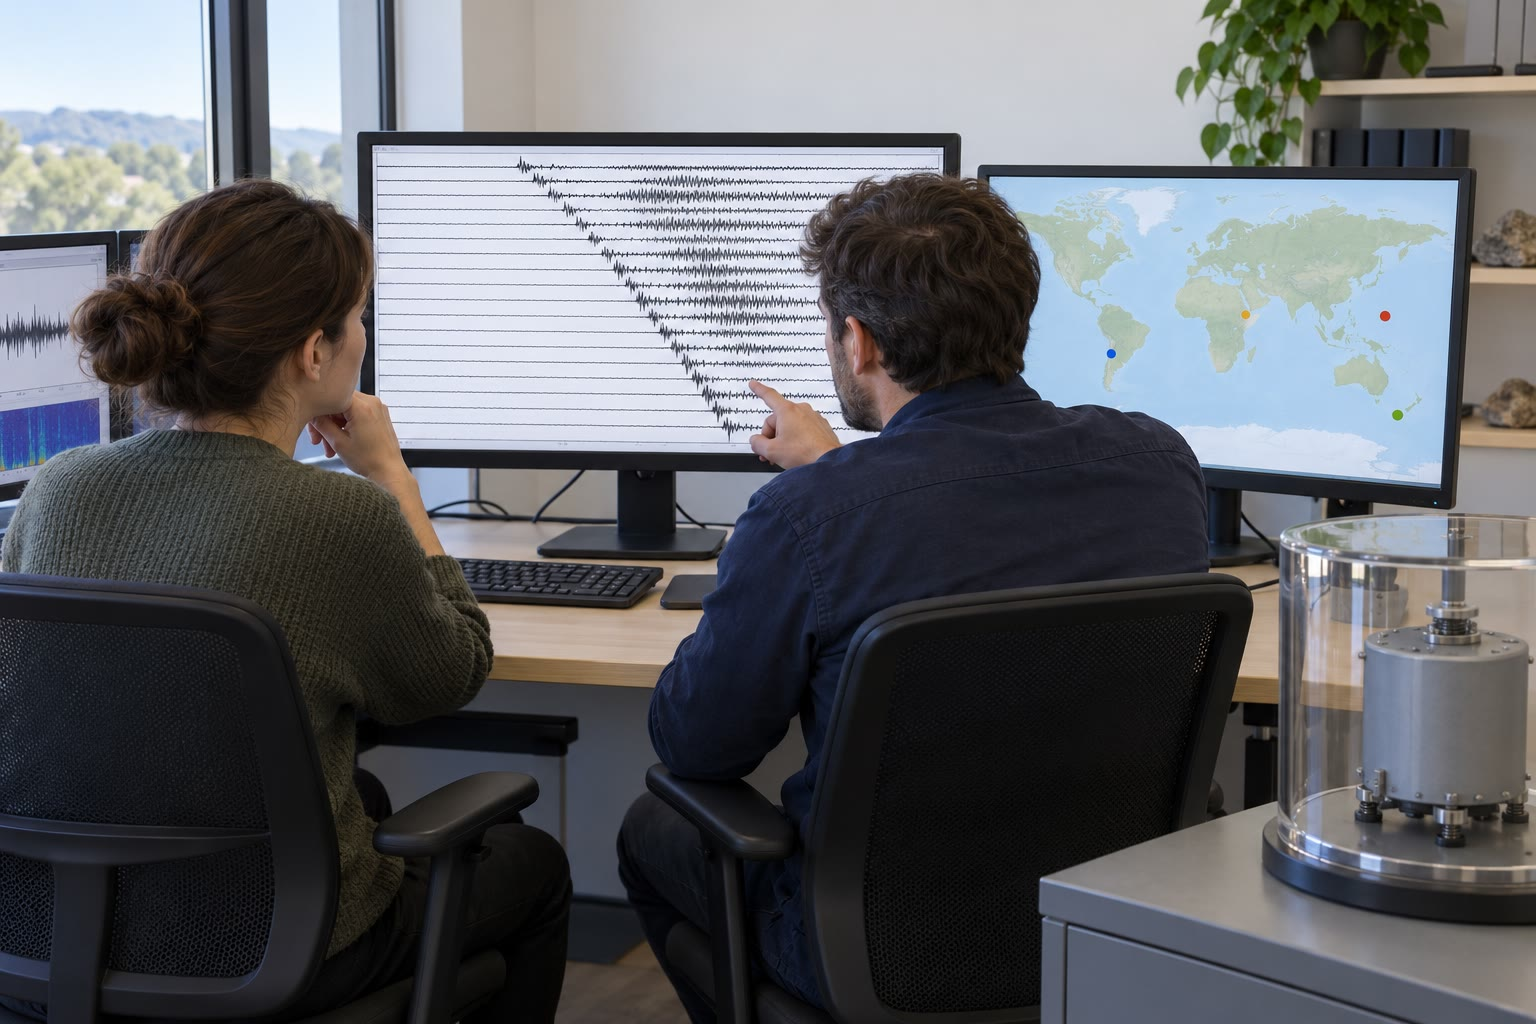
\includegraphics[width=\linewidth]{images/book3/ai/b1-seismic-analysis.jpg}

{\scriptsize Seismolog membaca bagian rekaman, jejak satu gempa bumi di stasiun yang diurutkan menurut jarak (ilustrasi AI).}
\end{minipage}
\end{inthelab}
% ledger: yvo:beachball

\section{Mengukur pembebanan: geodesi}\label{sec:b1:earthquake-source:geodesy}

Di antara gempa bumi, sesar yang terkunci tak terlihat oleh seismometer, tetapi tanah di sekitarnya bergerak. Stasiun penentuan posisi satelit permanen mengukur gerak itu, dan cara kecepatan mereka berubah melintasi sesar memberi tahu seberapa dalam sesar itu terkunci.

\begin{definition}[Kedalaman penguncian]\label{def:b1:earthquake-source:locking-depth}
\emph{Kedalaman penguncian}\index{kedalaman penguncian} sebuah sesar adalah kedalaman sampai mana ia terkunci di antara gempa bumi, sesar di bawahnya tergelincir mantap pada laju jangka panjang; ia adalah kedalaman bagian sesar yang akan tergelincir dalam gempa bumi berikutnya.
\end{definition}
% ledger: usgs:pp1515-thatcher

\begin{proposition}[Kecepatan antaseismik melintasi sesar geser-mendatar]\label{prop:b1:earthquake-source:interseismic}
Misalkan sebuah \omterm{def:b1:faults-folds-fabrics:fault-types}{sesar geser-mendatar} vertikal dalam setengah-ruang elastik terkunci dari permukaan hingga kedalaman $D$, dan meluncur pada laju $V$ di bawahnya. Kecepatan permukaan sejajar sesar, pada jarak $x$ darinya, adalah
\[
  v(x) = \frac{V}{\pi}\arctan\frac{x}{D} .
\]
Jika sesar kemudian tergelincir sebesar $s$ dari permukaan hingga kedalaman $D$ dalam gempa bumi, permukaan bergerak sebesar $u(x) = (s/\pi)\arctan(D/x)$ untuk $x > 0$, dan sebesar $-u(-x)$ untuk $x < 0$.
\end{proposition}
\admitted

Model ini, dari Savage dan Burford, adalah bentuk paling sederhana dari \omterm{def:b1:earthquake-source:seismic-cycle}{rebound elastik}, dan kurva pagar pada gambar pertama. Sifat-sifatnya mengikuti dari rumusnya.

\begin{proposition}[Membaca profil antaseismik]\label{prop:b1:earthquake-source:profile}
Dalam model \cref{prop:b1:earthquake-source:interseismic}:
\begin{enumerate}[label=(\alph*)]
  \item jauh dari sesar kecepatannya menuju $\pm V/2$, kedua lempeng bergerak sebesar $V$ satu sama lain;
  \item setengah dari perubahan kecepatan melintasi sesar terjadi dalam jarak $D$ darinya: $v(\pm D) = \pm V/4$;
  \item laju \omterm{def:b1:stress-strain-rheology:strain}{regangan geser} permukaan, $\mathrm dv/\mathrm dx$, terbesar pada sesar, tempat ia sama dengan $V/(\pi D)$;
  \item jika sesar, setelah dibebani selama waktu $t$, tergelincir sebesar $s = Vt$ dalam gempa bumi, tanah berakhir bergeser sebesar $\pm s/2$ di mana-mana pada kedua sisinya: siklus itu tidak meninggalkan lengkungan permanen, hanya pergeseran $s$ pada sesar.
\end{enumerate}
\end{proposition}

\begin{proof}
(a) $\arctan(x/D) \to \pm\pi/2$ ketika $x \to \pm\infty$. (b) $\arctan 1 = \pi/4$, sehingga $v(D) = V/4$, dan $v$ ganjil. (c) $\mathrm dv/\mathrm dx = (V/\pi D)/(1 +
x^2/D^2)$, terbesar pada $x = 0$. (d) Untuk $x > 0$, pembebanan telah menggerakkan tanah sebesar $t\,v(x) = (s/\pi)\arctan(x/D)$ dan gempa bumi sebesar $(s/\pi)\arctan(D/x)$; karena $\arctan y + \arctan(1/y) = \pi/2$ untuk $y > 0$, jumlahnya adalah $s/2$. Hal yang sama berlaku dengan tanda terbalik untuk $x < 0$.
\end{proof}

Sifat (b) memberi \omterm{def:b1:earthquake-source:locking-depth}{kedalaman penguncian} dari profil stasiun: itu adalah jarak dari sesar tempat kecepatannya telah berubah sebesar seperempat $V$ dari nilainya di sesar. Penguncian dangkal memusatkan regangan dekat sesar (gambar di bawah), penguncian dalam menyebarkannya di sabuk yang lebar. Sepanjang sistem San Andreas, \omterm{def:b1:earthquake-source:locking-depth}{kedalaman penguncian} yang ditemukan dari geodesi berkisar dari hampir 0, pada segmen yang merayap, hingga \qty{26}{km}, dan sesuai dengan kedalaman gempa bumi: bagian yang terkunci adalah \omterm{def:b1:stress-strain-rheology:strength-envelope}{lapisan seismogenik} \cref{ch:b1:stress-strain-rheology}. Untuk laju pergeseran \qty{34}{mm.yr^{-1}} dan \omterm{def:b1:earthquake-source:locking-depth}{kedalaman penguncian} \qty{15}{km}, laju \omterm{def:b1:stress-strain-rheology:strain}{regangan geser} pada sesar adalah $\num{0.034}/(\pi\times\num{15000}) = \num{7.2e-7}$ per tahun, yang membengkokkan garis melintasi sesar kurang dari satu milimeter per kilometer dalam setahun, namun menyimpan, dalam dua abad, beberapa meter pergeseran gempa bumi besar.
% ledger: sk:mu-locking, usgs:pp1515-wallace, usgs:pp1515-thatcher

\begin{omfigure}
\begin{tikzpicture}[font=\small]
\begin{axis}[omrecord, width=11cm, height=5.6cm, xmin=-100, xmax=100, ymin=-19, ymax=19,
    xlabel={jarak dari sesar $x$ (km)}, ylabel={kecepatan $v$ (\unit{mm.yr^{-1}})},
    legend style={font=\scriptsize, at={(0.02,0.96)}, anchor=north west}, legend cell align=left]
  \addplot[omDef, line width=0.9pt, dashed] table[x=x, y=v5] {figdata/out/bachelor-1-interseismic-profiles.dat};
  \addplot[omThm, line width=1.1pt] table[x=x, y=v15] {figdata/out/bachelor-1-interseismic-profiles.dat};
  \addplot[omProp, line width=0.9pt, dotted] table[x=x, y=v25] {figdata/out/bachelor-1-interseismic-profiles.dat};
  \legend{$D = \qty{5}{km}$, $D = \qty{15}{km}$, $D = \qty{25}{km}$}
  \draw[black!50, dashed] (axis cs:-100,17) -- (axis cs:100,17);
  \draw[black!50, dashed] (axis cs:-100,-17) -- (axis cs:100,-17);
  \node[anchor=north west, font=\scriptsize] at (axis cs:-30,17) {$+V/2$};
  \node[anchor=south west, font=\scriptsize] at (axis cs:30,-17) {$-V/2$};
  \draw[black!60] (axis cs:0,-19) -- (axis cs:0,19);
  \node[anchor=east, font=\scriptsize] at (axis cs:-1,5) {sesar};
\end{axis}
\end{tikzpicture}
\par\smallskip{\small Kecepatan tanah sejajar \omterm{def:b1:faults-folds-fabrics:fault-types}{sesar geser-mendatar} yang terkunci, relatif terhadap jejak sesar, untuk laju pergeseran $V = \qty{34}{mm.yr^{-1}}$, yaitu milik sesar San Andreas di Wallace Creek, dan tiga \omterm{def:b1:earthquake-source:locking-depth}{kedalaman penguncian} (\cref{prop:b1:earthquake-source:interseismic}). Makin dangkal penguncian, makin sempit sabuk tempat kecepatan itu berubah.}
\label{fig:b1:earthquake-source:interseismic}
\end{omfigure}
% ledger: usgs:pp1515-wallace

Penentuan posisi satelit mengukur tanah di beberapa stasiun. Satelit radar mengukurnya di mana-mana: dua citra radar dari daerah yang sama, diambil dari orbit yang sama pada waktu berbeda, dibandingkan gelombang demi gelombang, dan selisih fasenya memetakan perubahan jarak antara tanah dan satelit, titik demi titik, berjarak seratus meter, tanpa jaringan stasiun yang dipasang sebelumnya. Peta pertama dari gempa bumi besar California pada 1992 memperlihatkan perpindahan koseismiknya dalam satu gambar dan sesuai dengan pergeseran yang diukur di lapangan dan dengan survei; tekniknya, interferometri radar, termasuk dalam volume Tahun ke-3.
% ledger: massonnet:1993

\section{Seberapa sering: hukum Gutenberg--Richter}\label{sec:b1:earthquake-source:gr}

Gempa bumi kecil jauh lebih umum daripada yang besar, dengan cara yang sangat teratur.

\begin{proposition}[Hukum Gutenberg--Richter]\label{prop:b1:earthquake-source:gutenberg-richter}
Dalam suatu wilayah dan periode\index{hukum Gutenberg--Richter}, jumlah $N$ gempa bumi dengan magnitudo sedikitnya
$M$ mengikuti
\[
  \log_{10} N = a - bM ,
\]
untuk setiap $M$ di atas \omterm{def:b1:earthquake-source:b-value}{magnitudo kelengkapan} katalog, dengan konstanta $a$ dan $b$ yang bergantung pada wilayah; $b$ dekat dengan 1 di kebanyakan wilayah aktif.
\end{proposition}
\admitted
% ledger: fd:1993, gr:1944

Hukum ini adalah hasil pengamatan, diterbitkan oleh Beno Gutenberg dan Charles Richter untuk California pada 1944 dan sejak itu ditemukan di mana-mana; belum ada teori yang menurunkannya, atau nilai $b$.
% ledger: gr:1944

\begin{definition}[Nilai-b, magnitudo kelengkapan]\label{def:b1:earthquake-source:b-value}
Konstanta $b$ dari \omterm{prop:b1:earthquake-source:gutenberg-richter}{hukum Gutenberg--Richter} suatu wilayah adalah \emph{nilai-b}\index{nilai-b}-nya. \emph{Magnitudo kelengkapan}\index{magnitudo kelengkapan} sebuah katalog adalah magnitudo terkecil di atas mana ia mencatat setiap gempa bumi di wilayah dan periode itu.
\end{definition}

\omterm{def:b1:earthquake-source:b-value}{Nilai-b} 1 berarti sepuluh kali lebih sedikit gempa bumi untuk setiap satuan magnitudo. Di bawah \omterm{def:b1:earthquake-source:b-value}{magnitudo kelengkapan}, jumlahnya kurang dari garis, karena gempa bumi kecil direkam oleh terlalu sedikit stasiun untuk dapat ditentukan lokasinya: hukum itu tampak melengkung, dan $b$ harus diukur di atasnya. Untuk seluruh Bumi, dibagi menjadi gempa dangkal, menengah dan dalam, nilai terukur berada antara 0.72 dan 1.34, tetapi nilai itu berbeda sebesar \qty{30}{\percent} atau lebih dari satu katalog, rentang magnitudo atau metode ke yang lain: nilai yang jauh dari 1 pertama-tama merupakan alasan untuk memeriksa katalog.
% ledger: fd:1993

\begin{omfigure}
\begin{tikzpicture}[font=\small]
\begin{axis}[omrecord, width=6.4cm, height=5.8cm, ymode=log, xmin=5.8, xmax=9.3, ymin=0.01, ymax=300,
    xlabel={magnitudo $M$}, ylabel={gempa bumi bermagnitudo $\ge M$ per tahun},
    log basis y=10, title={(a) frekuensi dan magnitudo}, title style={font=\small}]
  \addplot[omProp, line width=0.9pt, domain=5.8:9.3] table[x=M, y=rate] {figdata/out/bachelor-1-gutenberg_richter-fit.dat};
  \addplot[only marks, mark=*, mark size=1.3pt, omDef] table[x=M, y=rate] {figdata/out/bachelor-1-gutenberg_richter-counts.dat};
  \draw[black!50, dashed] (axis cs:7.5,0.01) -- (axis cs:7.5,300);
  \node[anchor=south west, font=\scriptsize, omProp] at (axis cs:8.45,0.5) {$b = 1.01$};
  \node[anchor=north west, font=\scriptsize, align=left] at (axis cs:7.55,200) {dicocokkan pada\\ $6.0 \le M \le 7.5$};
\end{axis}
\begin{axis}[omrecord, at={(7.6cm,0)}, width=6.4cm, height=5.8cm, xmin=5.8, xmax=9.3, ymin=0, ymax=1.05,
    xlabel={magnitudo $M$}, ylabel={bagian momen dari gempa bumi $\ge M$},
    title={(b) ke mana momen pergi}, title style={font=\small}]
  \addplot[const plot, omDef, line width=0.9pt] table[x=M, y=share] {figdata/out/bachelor-1-gutenberg_richter-moment.dat};
\end{axis}
\end{tikzpicture}
\par\smallskip{\small \num{7031} gempa bumi bermagnitudo 6 atau lebih di dunia, 1976--2025 (katalog Survei Geologi Amerika Serikat). (a) Jumlah tahunan gempa bumi dengan magnitudo sedikitnya $M$; garis itu adalah kecocokan kuadrat terkecil dari $\log_{10} N$ terhadap $M$ dari 6.0 hingga 7.5, tempat setiap hitungan melampaui 200: $\log_{10} N = 8.20 - 1.01\,M$ per tahun. Di atas magnitudo 8 peristiwa yang sedikit jatuh di bawah garis. (b) Bagian dari seluruh \omterm{def:b1:earthquake-source:moment}{momen seismik} yang dilepaskan oleh gempa bumi bermagnitudo sedikitnya $M$, setiap momen dihitung sebagai $10^{1.5M + 9.1}$\,\unit{N.m}: 40 gempa bumi bermagnitudo 8 atau lebih melepaskan \qty{63}{\percent} darinya.}
\label{fig:b1:earthquake-source:gutenberg-richter}
\end{omfigure}
% ledger: data:usgs-comcat (fit and shares computed in figdata/bachelor-1/gutenberg_richter.py)

Untuk katalog dunia dalam gambar, hukum dengan $a = 8.20$ dan $b = 1.01$ memprediksi 14 gempa bumi bermagnitudo 7 atau lebih per tahun, seperti yang teramati, dan 1.35 bermagnitudo 8 atau lebih, sedangkan 40 dalam lima puluh tahun, 0.8 per tahun, tercatat. Apakah gempa bumi terbesar memang lebih sedikit daripada garis, seperti yang disarankan ukuran sesar yang terbatas, atau hanya cukup jarang sehingga tidak tercatat dalam lima puluh tahun, tidak diselesaikan oleh peristiwa yang sedikit ini. Sekitar satu dari sembilan magnitudo dalam katalog ini adalah magnitudo gelombang permukaan atau gelombang badan, yang jenuh; peristiwa terbesar semuanya memiliki \omterm{def:b1:earthquake-source:mw}{magnitudo momen}.
% ledger: data:usgs-comcat

Gempa bumi kecil yang banyak tidak banyak berperan. Jumlahnya tumbuh sepuluh kali untuk setiap satuan magnitudo lebih kecil, tetapi momennya menyusut 31.6 kali.

\begin{proposition}[Gempa bumi terbesar melepaskan sebagian besar momen]\label{prop:b1:earthquake-source:largest}
Misalkan gempa bumi mengikuti \omterm{prop:b1:earthquake-source:gutenberg-richter}{hukum Gutenberg--Richter} dengan $b < 1.5$, hingga magnitudo terbesar $M_{\max}$, dan misalkan mereka dikelompokkan dalam bin selebar satu satuan magnitudo, dengan bin teratas berakhir pada $M_{\max}$. Maka gempa bumi dari bin teratas melepaskan lebih dari pecahan $1 - 10^{-(1.5 - b)}$ dari seluruh momen, berapa pun kecilnya magnitudo terkecil yang dihitung: lebih dari \qty{68}{\percent} untuk $b = 1$.
\end{proposition}

\begin{proof}
Misalkan bin dinomori $k = 0, 1, \dots, K$ dari yang terkecil, bin $k$ berjalan dari $M_k$ hingga $M_k + 1$, dengan $M_{k+1} = M_k + 1$. Menurut hukum, jumlah gempa bumi dalam bin $k$ adalah $10^{a - bM_k} - 10^{a - b(M_k+1)} =
10^{a - bM_k}(1 - 10^{-b})$; menurut \cref{prop:b1:earthquake-source:moment-steps} momen tiap gempa berada antara $10^{1.5M_k + 9.1}$ dan $10^{1.5}$ kali itu, dan karena setiap bin adalah bin sebelumnya yang digeser satu satuan, momen bin $k$ adalah $C q^k$ untuk konstanta $C$ dan rasio $q = 10^{-b}\times10^{1.5} = 10^{1.5 - b} > 1$. Jumlahnya adalah deret geometri
\[
  S = C(1 + q + \dots + q^K) = C\,\frac{q^{K+1} - 1}{q - 1} ,
\]
dan bagian bin teratas adalah
\[
  \frac{C q^K}{S} = \frac{q^K (q - 1)}{q^{K+1} - 1}
  > \frac{q^K (q - 1)}{q^{K+1}} = 1 - \frac1q = 1 - 10^{-(1.5 - b)} .
\]
Untuk $b = 1$, $1 - 10^{-0.5} = 0.684$.
\end{proof}

Di katalog dunia, bagian ini berorde seperti ini: satuan magnitudo teratas, dari 8.1 hingga 9.1, melepaskan lebih dari separuh momen lima puluh tahun, dan dua gempa bumi terbesar, Sumatra--Andaman 2004 dan Tohoku 2011, dengan magnitudo 9.1, melepaskan \qty{29}{\percent} darinya sendiri. Momen yang harus dilepaskan sebuah batas lempeng ditentukan oleh laju pergeserannya; proposisi mengatakan bahwa ia dilepaskan hampir seluruhnya dalam gempa bumi terbesarnya, dan bahwa gempa-gempa kecil yang banyak, berapa pun seringnya, tidak meringankan sesar dari yang besar berikutnya.
% ledger: data:usgs-comcat, usgs:sumatra-mt, usgs:tohoku-mt

\section{Latihan}

\begin{exercise}[$\star$]\label{exo:b1:earthquake-source:1}
(a) Hitung \omterm{def:b1:earthquake-source:mw}{magnitudo momen} gempa bumi dengan \omterm{def:b1:earthquake-source:moment}{momen seismik} \qty{4e17}{N.m}. (b) Gempa Tohoku memiliki $M_0 = \qty{5.59e22}{N.m}$: periksa magnitudonya. (c) \omterm{def:b1:earthquake-source:moment}{Momen seismik} apa yang dimiliki gempa bumi bermagnitudo 7.0?
% ledger: usgs:tohoku-mt
\end{exercise}

\begin{exercise}[$\star$]\label{exo:b1:earthquake-source:2}
Sebuah \omterm{def:b1:faults-folds-fabrics:fault-types}{sesar geser-mendatar} dibebani pada \qty{25}{mm.yr^{-1}}, dan gempa-gempanya masing-masing tergelincir sekitar \qty{3}{m}. (a) Berapa \omterm{def:b1:earthquake-source:seismic-cycle}{interval perulangannya} jika sesar sepenuhnya terkunci di antara mereka? (b) Dan jika setengah laju pergeseran diambil oleh rayapan mantap?
\end{exercise}

\begin{exercise}[$\star$]\label{exo:b1:earthquake-source:3}
Berapa kali lebih besar \omterm{def:b1:earthquake-source:moment}{momen seismik} gempa bumi bermagnitudo 7.4 daripada gempa bumi bermagnitudo 6.2? Berapa gempa bumi bermagnitudo 6.2 yang akan melepaskan momen yang sama?
\end{exercise}

\begin{exercise}[$\star$]\label{exo:b1:earthquake-source:4}
Di suatu wilayah dengan $b = 1$, seribu gempa bumi bermagnitudo 3 atau lebih tercatat setiap tahun. Berapa yang bermagnitudo 5 atau lebih, dan bermagnitudo 6 atau lebih, diharapkan setiap tahun? Berapa rata-rata waktu antara gempa bumi bermagnitudo 7 atau lebih?
\end{exercise}

\begin{exercise}[$\star\star$]\label{exo:b1:earthquake-source:5}
Gempa bumi 1906 memecah sesar San Andreas sepanjang sekitar \qty{430}{km}. (a) Dengan anggapan rekahan mencapai kedalaman \qty{15}{km} dengan pergeseran rata-rata \qty{4}{m}, dan $\mu = \qty{30}{GPa}$, hitung \omterm{def:b1:earthquake-source:moment}{momen seismik} dan \omterm{def:b1:earthquake-source:mw}{magnitudo momennya}. (b) Berapa banyak magnitudo berubah jika rekahan hanya \qty{10}{km} dalamnya? (c) Mana dari kedua perkiraan itu yang lebih dekat dengan 7.9?
% ledger: pp1515:1906, usgs:hist-mw
\end{exercise}

\begin{exercise}[$\star\star$]\label{exo:b1:earthquake-source:6}
Rekahan gempa Tohoku memiliki panjang sekitar \qty{400}{km} dan lebar \qty{150}{km}, dan momennya \qty{5.59e22}{N.m}. (a) Hitung pergeserannya rata-rata dengan $\mu = \qty{30}{GPa}$. (b) Lempeng Pasifik menunjam di bawah Jepang pada sekitar \qty{83}{mm.yr^{-1}}: berapa lama waktu yang diperlukan untuk mengumpulkan pergeseran ini jika antarmukanya terkunci sepenuhnya? (c) Dan jika fraksi yang terkunci 0.8, atau 0.5?
% ledger: usgs:tohoku-mt, usgs:tohoku-summary
\end{exercise}

\begin{exercise}[$\star\star$]\label{exo:b1:earthquake-source:7}
Satu \omterm{def:b1:earthquake-source:focal-mechanism}{bidang nodal} gempa Sumatra--Andaman 2004 berjurus $329$, miring \ang{8} dan \omterm{def:b1:faults-folds-fabrics:fault-elements}{rake} \ang{110}. (a) Tuliskan $\mathbf n$ dan $\mathbf d$ dalam komponen timur, utara dan atas. (b) Cari \omterm{def:b1:geological-maps:attitude}{jurus}, \omterm{def:b1:geological-maps:attitude}{kemiringan} dan \omterm{def:b1:faults-folds-fabrics:fault-elements}{rake} \omterm{def:b1:earthquake-source:focal-mechanism}{bidang bantu}. (c) Cari arah dan \omterm{def:b1:field-lab-methods-1:trend-plunge}{penunjaman} \omterm{def:b1:earthquake-source:focal-mechanism}{sumbu P} dan T. (d) Bidang mana yang merupakan sesar, dan sesar jenis apa itu?
% ledger: usgs:sumatra-mt
\end{exercise}

\begin{exercise}[$\star\star$]\label{exo:b1:earthquake-source:8}
Sebuah sesar vertikal berjurus $045$ tergelincir secara \omterm{def:b1:faults-folds-fabrics:fault-types}{dekstral}. (a) Untuk gelombang yang meninggalkan fokus secara horizontal menuju stasiun-stasiun yang berada tepat di utara, timur, selatan dan barat, yang mana datang sebagai dorongan dan yang sebagai tarikan? (b) Berikan arah \omterm{def:b1:earthquake-source:focal-mechanism}{sumbu P} dan T. (c) Tunjukkan bahwa pergeseran \omterm{def:b1:faults-folds-fabrics:fault-types}{sinistral} pada bidang vertikal yang berjurus $135$ memberi \omterm{def:b1:earthquake-source:focal-mechanism}{gerak pertama} yang sama.
\end{exercise}

\begin{exercise}[$\star\star$]\label{exo:b1:earthquake-source:9}
Melintasi \omterm{def:b1:faults-folds-fabrics:fault-types}{sesar geser-mendatar} yang terkunci, stasiun-stasiun jauh di kedua sisi bergerak sebesar \qty{40}{mm.yr^{-1}} relatif satu sama lain. Sebuah stasiun \qty{10}{km} dari sesar bergerak sebesar \qty{10}{mm.yr^{-1}} relatif terhadap jejak sesar. (a) Cari \omterm{def:b1:earthquake-source:locking-depth}{kedalaman penguncian}. (b) Prediksikan kecepatan stasiun \qty{30}{km} dari sesar. (c) Hitung laju \omterm{def:b1:stress-strain-rheology:strain}{regangan geser} pada sesar.
\end{exercise}

\begin{exercise}[$\star\star\star$]\label{exo:b1:earthquake-source:10}
(a) Tunjukkan bahwa, jika $b$ lebih besar dari 1.5, momen total gempa bumi suatu wilayah akan didominasi oleh yang terkecil. (b) Berapa bagian momen yang dilepaskan oleh satuan magnitudo teratas, paling sedikit, untuk $b = 0.8$? (c) Dengan $a = 8.20$ dan $b = 1.01$ per tahun untuk katalog dunia, berapa gempa bumi bermagnitudo 9 atau lebih yang akan diprediksi hukum dalam lima puluh tahun? Katalog 1976--2025 memuat dua; beri komentar.
% ledger: data:usgs-comcat
\end{exercise}

\begin{exercise}[$\star\star\star$]\label{exo:b1:earthquake-source:11}
Sebuah pagar lurus dibangun melintasi sesar \omterm{def:b1:faults-folds-fabrics:fault-types}{dekstral} terkunci dengan $V =
\qty{34}{mm.yr^{-1}}$ dan $D = \qty{15}{km}$. (a) Setelah 150 tahun, sebesar berapa tiang-tiang \qty{1}{km}, \qty{15}{km} dan \qty{50}{km} di timur sesar telah bergerak sepanjangnya, relatif terhadap tiang di sesar? (b) Sesar kemudian tergelincir sebesar seluruh defisit dalam gempa bumi. Berapa pergeserannya, dan sejauh mana masing-masing dari ketiga tiang bergerak selama gempa bumi? (c) Periksa bagian (d) dari \cref{prop:b1:earthquake-source:profile} pada ketiga tiang itu.
% ledger: usgs:pp1515-wallace
\end{exercise}

\begin{exercise}[$\star\star\star$]\label{exo:b1:earthquake-source:12}
Sebuah gempa bumi memiliki \omterm{def:b1:earthquake-source:focal-mechanism}{sumbu P} horizontal berarah $000$ dan \omterm{def:b1:earthquake-source:focal-mechanism}{sumbu T} horizontal berarah $090$. (a) Tunjukkan bahwa \omterm{def:b1:earthquake-source:focal-mechanism}{bidang nodalnya} vertikal dan berjurus $045$ dan $135$, dengan menggunakan $\mathbf n$, $\mathbf d = (\mathbf T \pm \mathbf P)/\sqrt2$. (b) Berikan arah pergeseran pada setiap bidang. (c) Jika sesar itu terbentuk sebagai sesar baru dalam batuan dengan $\phi = \ang{30}$, di bawah $\sigma_1$ sepanjang \omterm{def:b1:earthquake-source:focal-mechanism}{sumbu P}, pada \omterm{def:b1:geological-maps:attitude}{jurus} berapa ia akan terletak, dan mengapa \omterm{def:b1:earthquake-source:focal-mechanism}{sumbu P} hanya perkiraan $\sigma_1$? (d) Sebuah sesar terpetakan di dekatnya berjurus $040$. \omterm{def:b1:earthquake-source:focal-mechanism}{Bidang nodal} mana yang kemungkinan adalah sesar, dan apa arah pergeserannya?
\end{exercise}

\section{Masalah: gempa bumi besar berikutnya pada sesar terkunci}

\begin{problem}[{Soal akhir pekan --- segmen terkunci dari batas lempeng geser-mendatar, dari pembebanannya dan gempa-gempa masa lalunya hingga magnitudo yang berikutnya}]
\label{pb:b1:earthquake-source:1}
% values: calc/ch18.py; an invented fault (the numbers are of a realistic order)
Sebuah \omterm{def:b1:faults-folds-fabrics:fault-types}{sesar geser-mendatar} vertikal yang lurus membentuk batas antara dua lempeng. Satu segmennya, sepanjang \qty{250}{km}, terkunci; gempa-gempanya mulai tidak lebih dalam dari \qty{15}{km}. Parit yang digali melintasinya menanggalkan empat gempa bumi besar terakhirnya sekitar tahun 1050, 1290, 1480 dan 1712, dengan pergeseran \num{7.0}, \num{6.0}, \num{5.5} dan \qty{7.5}{m}. Stasiun permanen yang jauh dari sesar di kedua sisinya bergerak sebesar \qty{30}{mm.yr^{-1}} relatif satu sama lain. Ambil $\mu =
\qty{30}{GPa}$, tahun 2025 sebagai masa kini, dan berikan magnitudo hingga 0.01.

\medskip
\noindent\textbf{Bagian I --- Pembebanan.}
\begin{enumerate}
  \item Hitung interval antara keempat gempa bumi dan rata-ratanya.
  \item Hitung rata-rata pergeseran, dan \omterm{def:b1:earthquake-source:seismic-cycle}{interval perulangan} yang diimplikasikannya dengan \cref{prop:b1:earthquake-source:recurrence} untuk sesar yang terkunci sepenuhnya.
  \item Hitung laju pergeseran yang diimplikasikan oleh parit saja, dari pergeseran ketiga gempa bumi terakhir dan waktu antara yang pertama dan yang terakhir. Bandingkan dengan laju geodetik.
  \item Berapa lama yang lalu gempa bumi terakhir terjadi, dan defisit pergeseran apa yang telah terkumpul sejak itu, jika segmen itu terkunci sepenuhnya?
  \item Bandingkan defisit ini dengan pergeseran di parit. Apakah gempa berikutnya sudah terlambat?
  \item Mengapa parit tidak dapat memberi tanggal bagi yang berikutnya?
\end{enumerate}

\medskip
\noindent\textbf{Bagian II --- Ukuran gempa bumi berikutnya.}
\begin{enumerate}[resume]
  \item Berapa luas bagian yang terkunci dari segmen itu?
  \item Hitung \omterm{def:b1:earthquake-source:moment}{momen seismik} gempa bumi yang akan melepaskan seluruh defisit itu.
  \item Hitung \omterm{def:b1:earthquake-source:mw}{magnitudo momen} gempa bumi 1712, dengan anggapan ia memecah luas yang sama dengan pergeseran parit sebagai pergeseran rata-rata.
  \item Dengan faktor berapa momen gempa bumi berikutnya melampaui 1712, dan berapa satuan magnitudo itu?
  \item Jika hanya setengah segmen yang pecah, dengan pergeseran yang sama, berapa magnitudonya?
  \item Berikan \omterm{def:b1:earthquake-source:moment}{momen seismik} yang dikumpulkan segmen setiap tahun.
\end{enumerate}

\medskip
\noindent\textbf{Bagian III --- Frekuensi dan energi.}
\begin{enumerate}[resume]
  \item Katalog regional mengikuti $\log_{10} N = 4.3 - M$ per tahun, dari semua sesar di wilayah itu. Berapa \omterm{def:b1:earthquake-source:b-value}{nilai-b-nya}, dan berapa gempa bumi bermagnitudo 5 atau lebih, dan 6 atau lebih, yang diberikannya setiap tahun?
  \item Berapa interval rata-rata antara gempa bumi bermagnitudo 7 atau lebih yang diberikannya, dan bermagnitudo 8 atau lebih?
  \item Bandingkan perulangan gempa bumi besar dari katalog dengan yang dari parit. Apa yang dikatakan perbedaan itu tentang penggunaan hukum gempa kecil untuk memperkirakan gempa besar?
  \item Gempa bumi bermagnitudo 5 hingga 8 dari hukum regional melepaskan, bersama-sama, sekitar \qty{5.5e17}{N.m} setahun. Berapa pecahan momen segmen itu?
  \item Berapa kali lebih banyak energi daripada gempa bumi bermagnitudo 6 yang akan dipancarkan gempa bumi besar berikutnya?
  \item Dengan \cref{prop:b1:earthquake-source:largest}, jelaskan mengapa gempa bumi sedang pada segmen itu tidak meringankannya.
\end{enumerate}

\medskip
\noindent\textbf{Bagian IV --- Kedalaman penguncian dari stasiun.}
\begin{enumerate}[resume]
  \item Sebuah profil stasiun melintasi segmen memberi, relatif terhadap jejak sesar, kecepatan $-11.6$, $-7.5$, $-3.1$, $3.1$, $7.5$ dan \qty{11.6}{mm.yr^{-1}} pada $x = -40$, $-15$, $-5$, $5$, $15$ dan \qty{40}{km}. Periksa bahwa profilnya antisimetris, dan berikan kecepatan yang diharapkan jauh dari sesar.
  \item Dari stasiun pada \qty{15}{km}, hitung \omterm{def:b1:earthquake-source:locking-depth}{kedalaman penguncian}.
  \item Hitung lagi dari stasiun pada \qty{5}{km} dan \qty{40}{km}, dan jelaskan perbedaan kecil itu.
  \item Bandingkan \omterm{def:b1:earthquake-source:locking-depth}{kedalaman penguncian} dengan kedalaman gempa bumi, dan katakan mengapa keduanya seharusnya sesuai.
  \item Hitung laju \omterm{def:b1:stress-strain-rheology:strain}{regangan geser} pada sesar.
  \item Hingga 0.01, berapa \omterm{def:b1:earthquake-source:mw}{magnitudo momen} gempa bumi yang akan melepaskan seluruh defisit pergeseran segmen itu?
\end{enumerate}
\end{problem}
